\chapter{TÁI HIỆN KẾT QUẢ VÀ ĐỊNH HƯỚNG CẢI TIẾN}

Chương này trình bày phần thực nghiệm độc lập của nhóm theo ba tầng tách biệt: \textbf{tái hiện bài báo}, \textbf{phân tích thành phần (ablation)} và \textbf{mở rộng/cải tiến}. Sự phân tách này đặc biệt quan trọng vì bài báo tập trung báo cáo kết quả của pipeline có xử lý mất cân bằng; trong khi nhóm còn đánh giá thêm mô hình trên tập kiểm tra giữ nguyên phân bố lớp. Hai loại kết quả này không được dùng để so sánh trực tiếp với nhau.

\section{Mục tiêu và nguyên tắc tái hiện}

Mục tiêu thứ nhất là tái dựng pipeline XGBoost của tác giả trên hai bộ dữ liệu và kiểm tra mức độ có thể lặp lại các kết quả đã công bố. Theo pipeline được nhóm tái dựng, Dataset 1 sử dụng SMOTE để xử lý mất cân bằng, còn Dataset 2 sử dụng Random UnderSampler. PCA sau đó được sử dụng để giảm chiều trước khi huấn luyện XGBoost.

Mục tiêu thứ hai là đánh giá từng thành phần của pipeline bằng ablation study. Nhóm lần lượt khảo sát mô hình cơ sở, tác động của PCA, xử lý mất cân bằng và tuning. Các bước này chưa được gọi là đề xuất cải tiến vì phần lớn là các thành phần đã thuộc pipeline gốc hoặc phục vụ mục tiêu tái hiện.

Mục tiêu thứ ba, sau khi đã có baseline tái hiện, là khảo sát các lựa chọn khác với pipeline gốc: SMOTENC và học có trọng số lớp trên Dataset 1; học có trọng số lớp trên Dataset 2; đồng thời khảo sát việc có/không PCA và lựa chọn threshold theo yêu cầu specificity. Đây mới là phần mở rộng phương pháp của nhóm.

\section{Quá trình tái dựng pipeline}

Thay vì chỉ báo cáo mô hình cuối cùng, nhóm lưu lại kết quả sau từng bước để xác định đóng góp của các thành phần. Bảng~\ref{tab:model_progression} trình bày chuỗi thực nghiệm trên tập kiểm tra giữ nguyên phân bố lớp. Đây là đánh giá bổ sung của nhóm nhằm quan sát hành vi mô hình trong điều kiện lớp mất cân bằng ban đầu; các con số trong bảng không được dùng để so trực tiếp với kết quả công bố của tác giả.

\begin{table}[H]
\centering
\scriptsize
\caption{Diễn biến kết quả qua các bước tái dựng pipeline}
\label{tab:model_progression}
\resizebox{\linewidth}{!}{%
\begin{tabular}{llrrrrrr}
\toprule
\textbf{Dữ liệu} & \textbf{Bước} & \textbf{Accuracy} & \textbf{Precision} & \textbf{Recall} & \textbf{F1} & \textbf{ROC-AUC} & \textbf{MCC}\\
\midrule
Dataset 1 & Baseline, không PCA & 0,9501 & 0,4286 & 0,0600 & 0,1053 & 0,8307 & 0,1462\\
Dataset 1 & Baseline + PCA & 0,9491 & 0,3333 & 0,0400 & 0,0714 & 0,8011 & 0,1013\\
Dataset 1 & Balancing & 0,9119 & 0,1296 & 0,1400 & 0,1346 & 0,7880 & 0,0884\\
Dataset 1 & Balancing + PCA & 0,8249 & 0,1272 & 0,4400 & 0,1973 & 0,7716 & 0,1637\\
Dataset 1 & Balancing + PCA + tuning & 0,7818 & 0,1554 & 0,7800 & 0,2591 & 0,8118 & 0,2816\\
\midrule
Dataset 2 & Baseline, không PCA & 0,9612 & 0,9152 & 0,0986 & 0,1780 & 0,9319 & 0,2934\\
Dataset 2 & Baseline + PCA & 0,9638 & 0,9723 & 0,1538 & 0,2656 & 0,9641 & 0,3792\\
Dataset 2 & Balancing & 0,8166 & 0,1807 & 0,9360 & 0,3030 & 0,9376 & 0,3639\\
Dataset 2 & Balancing + PCA & 0,8572 & 0,2262 & 0,9722 & 0,3670 & 0,9714 & 0,4304\\
Dataset 2 & Balancing + PCA + tuning & 0,9664 & 0,5590 & 0,9944 & 0,7157 & 0,9976 & 0,7322\\
\bottomrule
\end{tabular}}
\end{table}

Trên Dataset 1, baseline đạt Accuracy gần 95\% nhưng Recall chỉ 6\%, cho thấy Accuracy cao chủ yếu do lớp không đột quỵ chiếm ưu thế. Khi hoàn thiện balancing, PCA và tuning, Recall tăng lên 78\%, F1 tăng từ 0,1053 lên 0,2591 và MCC tăng từ 0,1462 lên 0,2816, đổi lại Accuracy giảm. Trên Dataset 2, tác động còn rõ hơn: Recall tăng từ 0,0986 lên 0,9944, F1 từ 0,1780 lên 0,7157 và MCC từ 0,2934 lên 0,7322. Kết quả này cho thấy xử lý mất cân bằng là thành phần thiết yếu nếu mục tiêu là phát hiện lớp đột quỵ thay vì chỉ tối đa hóa Accuracy.

\begin{figure}[H]
    \centering
    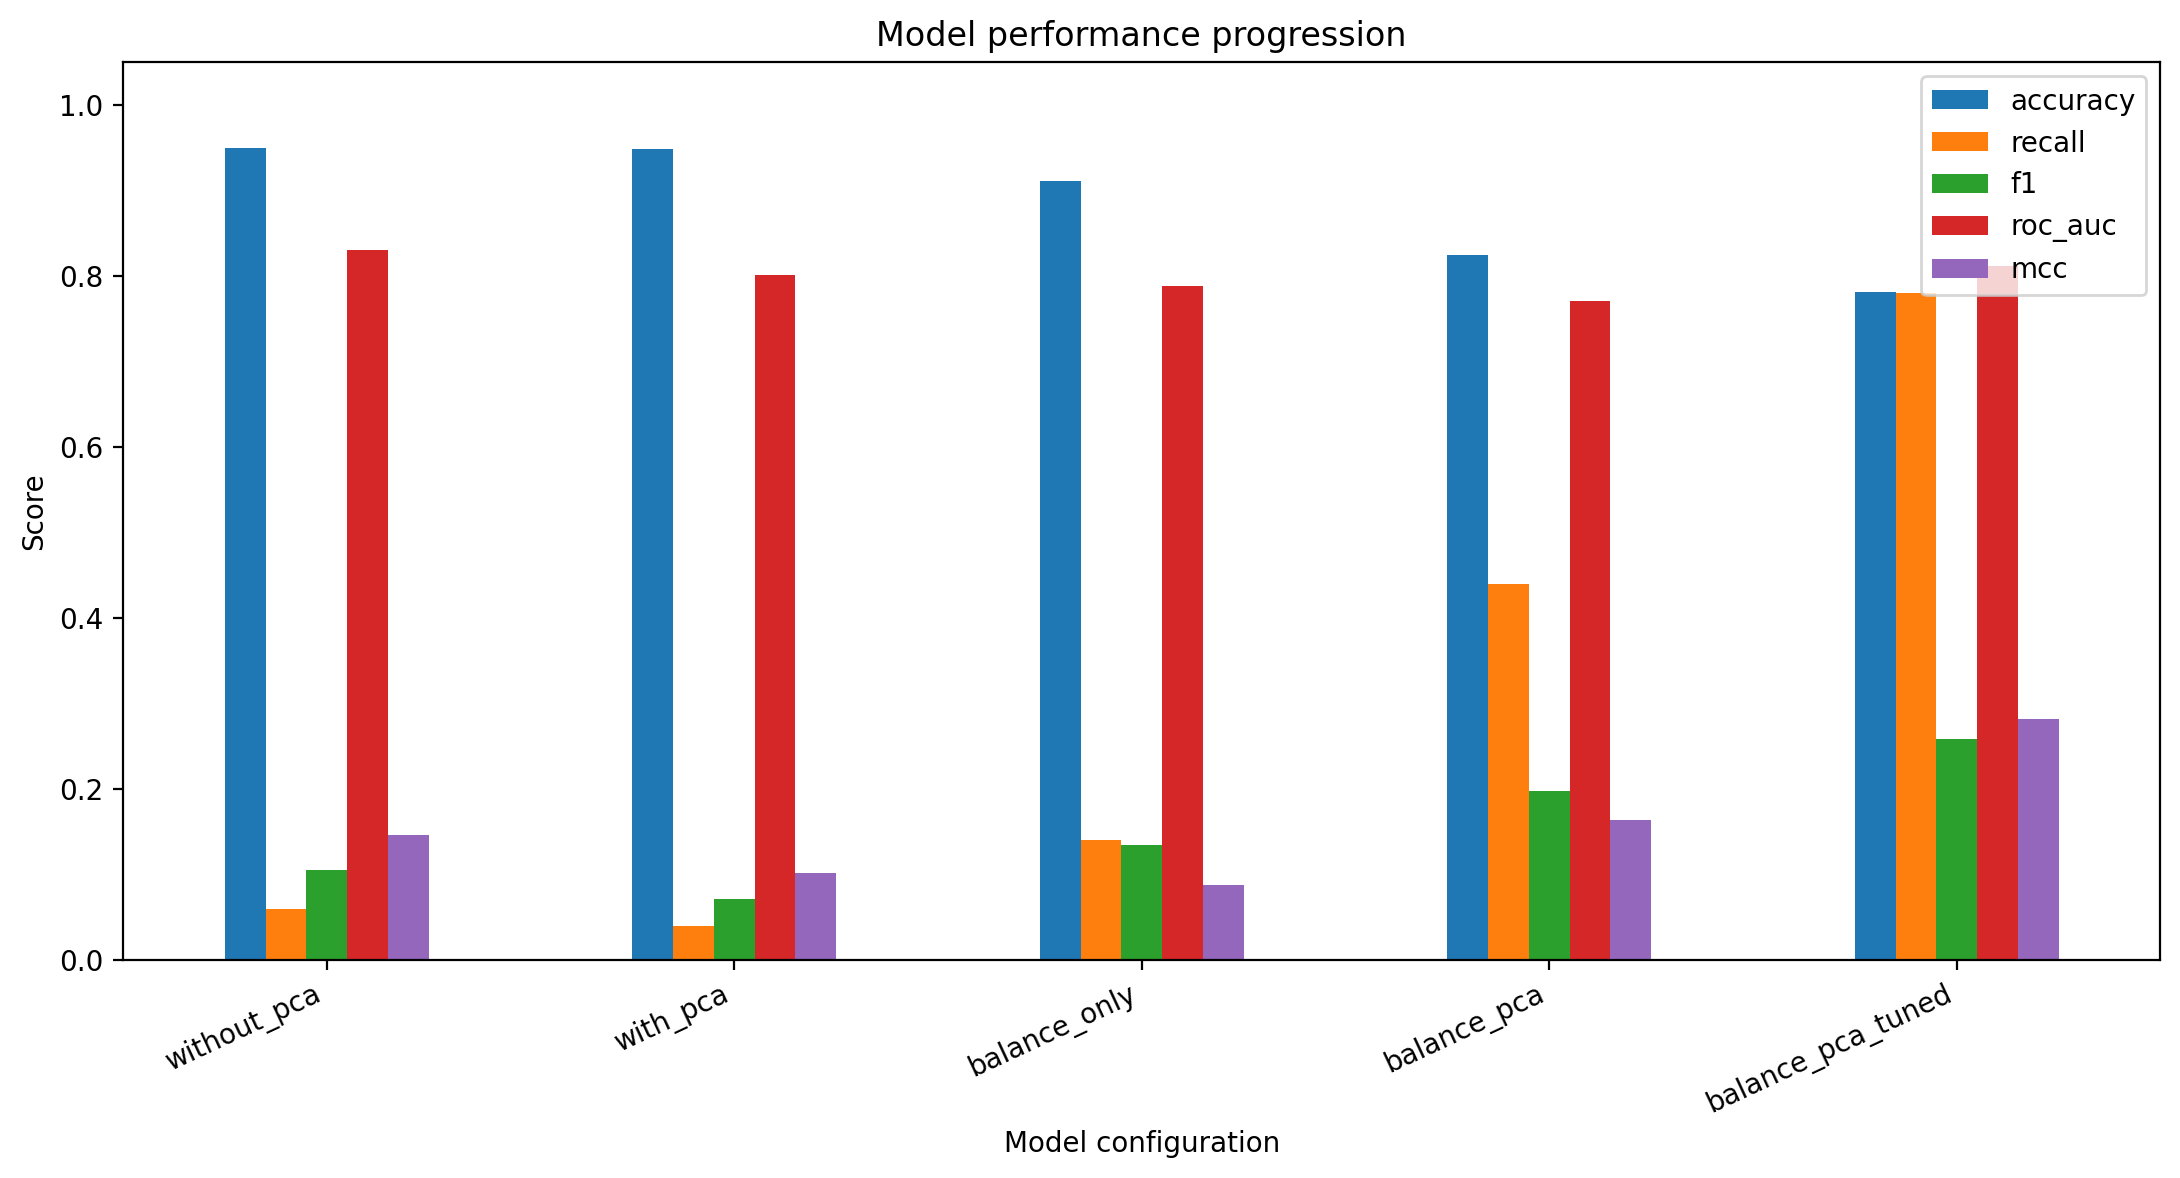
\includegraphics[width=0.90\textwidth]{../results/final_reproduction/dataset1_model_progression.png}
    \caption{Diễn biến hiệu năng qua các bước tái dựng pipeline trên Dataset 1.}
    \label{fig:d1_model_progression}
\end{figure}

\begin{figure}[H]
    \centering
    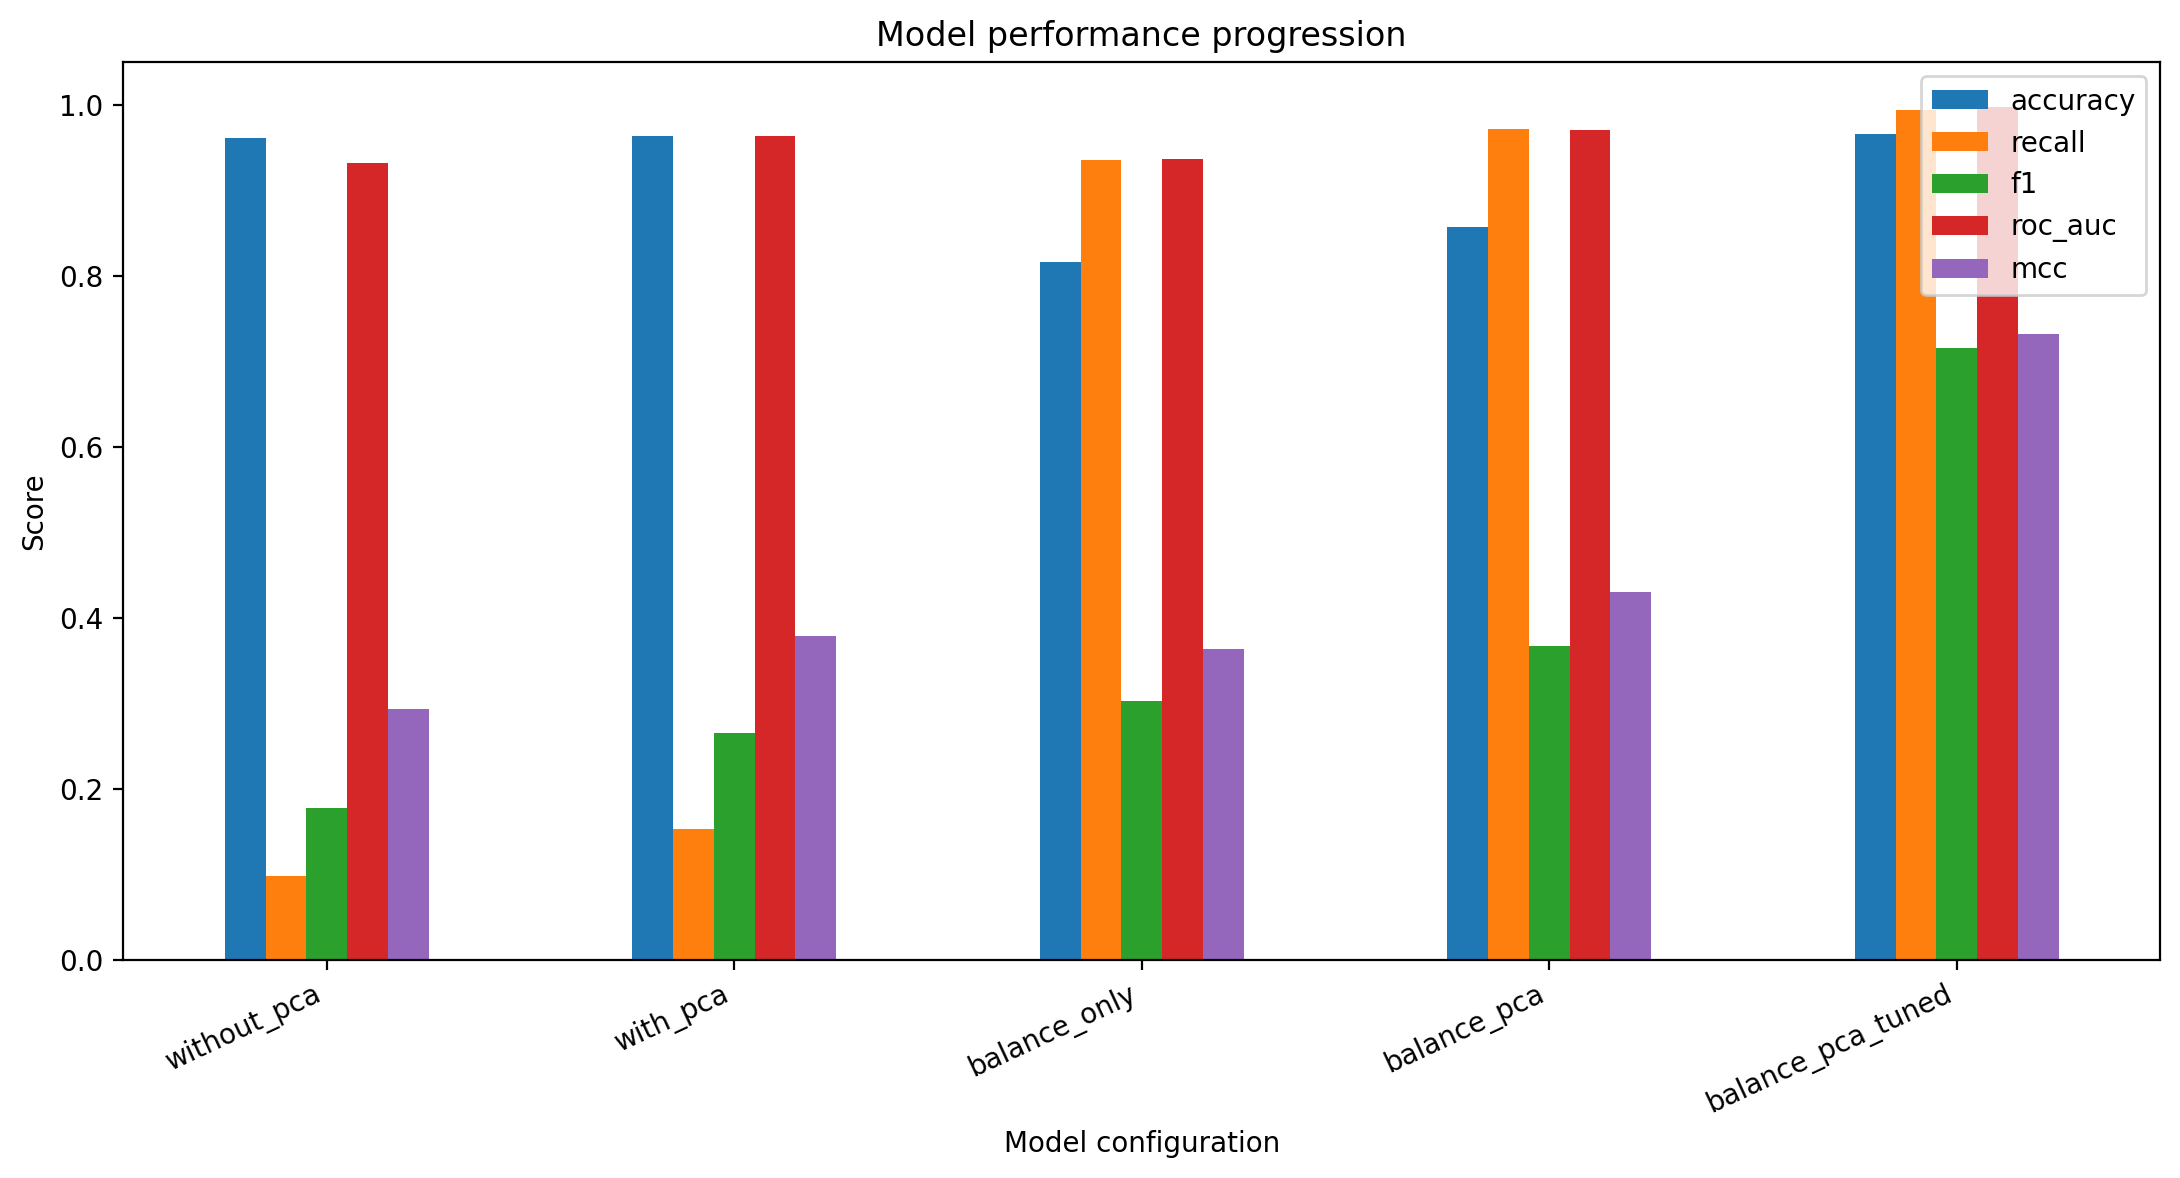
\includegraphics[width=0.90\textwidth]{../results/final_reproduction/dataset2_model_progression.png}
    \caption{Diễn biến hiệu năng qua các bước tái dựng pipeline trên Dataset 2.}
    \label{fig:d2_model_progression}
\end{figure}

Hai hình trên được trình bày riêng cho từng bộ dữ liệu. Nhóm không gộp các metric của Dataset 1 và Dataset 2 vào cùng một hình vì hai bộ dữ liệu khác nhau đáng kể về quy mô, nguồn dữ liệu và độ khó dự đoán.

\section{Kết quả tái hiện so với bài báo}

Sau khi hoàn thiện pipeline theo cách hiểu từ bài báo, Dataset 1 sử dụng SMOTE và giữ 11 thành phần PCA, giải thích khoảng 96,50\% phương sai. Dataset 2 sử dụng Random UnderSampler và giữ 11 thành phần PCA, giải thích khoảng 95,86\% phương sai. Bảng~\ref{tab:reproduction_comparison} chỉ đối chiếu các chỉ số có giá trị tương ứng được bài báo công bố.

\begin{table}[H]
\centering
\caption{Đối chiếu kết quả công bố và kết quả tái hiện}
\label{tab:reproduction_comparison}
\begin{tabular}{llrrr}
\toprule
\textbf{Dữ liệu} & \textbf{Chỉ số} & \textbf{Bài báo} & \textbf{Tái hiện} & \textbf{Chênh lệch}\\
\midrule
Dataset 1 & CV Accuracy & 0,9532 & 0,7652 & -0,1880\\
Dataset 2 & CV Accuracy & 0,9903 & 0,9654 & -0,0249\\
Dataset 2 & MCC & 0,9634 & 0,7322 & -0,2312\\
Dataset 2 & Cohen's Kappa & 0,9632 & 0,6993 & -0,2639\\
\bottomrule
\end{tabular}
\end{table}

Dataset 2 tái hiện gần kết quả công bố hơn về Accuracy, nhưng MCC và Cohen's Kappa vẫn thấp hơn đáng kể. Dataset 1 còn sai khác lớn. Do đó, nhóm không tuyên bố đã tái lập hoàn toàn các con số của tác giả. Một số chi tiết triển khai như thời điểm resampling, cách chia dữ liệu, encoding, random seed, hyperparameter và cách tổng hợp chỉ số cross-validation có thể tạo ra sai khác.

Quan trọng hơn, bài báo không cung cấp một bộ kết quả tương ứng trên tập test giữ nguyên phân bố lớp để nhóm đối chiếu trực tiếp với phần đánh giá bổ sung của mình. Vì vậy, các kết quả trên test giữ nguyên phân bố lớp trong phần sau chỉ được dùng để so sánh \textbf{các cấu hình của nhóm với nhau trên cùng một giao thức}.

\section{Ablation: vai trò của balancing, PCA và tuning}

Kết quả ở Bảng~\ref{tab:model_progression} cho phép rút ra ba nhận xét. Thứ nhất, Accuracy đơn lẻ không phù hợp để lựa chọn mô hình trong bài toán mất cân bằng: baseline Dataset 1 có Accuracy 0,9501 nhưng bỏ sót gần như toàn bộ ca đột quỵ. Thứ hai, PCA không phải lúc nào cũng cải thiện mô hình nếu đứng riêng lẻ; trên Dataset 1, thêm PCA vào baseline làm Recall giảm từ 0,06 xuống 0,04. Thứ ba, tác động lớn nhất xuất hiện khi balancing được kết hợp với PCA và tuning, đặc biệt ở Recall, F1 và MCC.

Do đó, trong phần còn lại của chương, SMOTE trên Dataset 1 và Random UnderSampler trên Dataset 2 được xem là \textbf{baseline xử lý mất cân bằng theo pipeline tái hiện}, không được gọi là đề xuất mới. Thử nghiệm có/không PCA được xem là ablation. Những phương pháp thay thế balancing hoặc thay đổi quy tắc quyết định mới được xem là hướng mở rộng của nhóm.

\section{Mở rộng phương pháp xử lý mất cân bằng}

Để so sánh công bằng, nhóm chia train/test trước khi ước lượng các tham số tiền xử lý. Imputation, chuẩn hóa, encoding, PCA và resampling chỉ được fit trên dữ liệu huấn luyện hoặc bên trong từng fold. Tập test giữ nguyên phân bố lớp và không được resample. Ngưỡng phân loại được lựa chọn từ validation hoặc dự đoán out-of-fold rồi khóa trước khi đánh giá test.

\subsection{Dataset 1: từ SMOTE sang SMOTENC và cost-sensitive learning}

SMOTE là phương pháp thuộc baseline tái hiện của Dataset 1. Nhóm mở rộng bằng hai hướng: \textbf{SMOTENC}, nhằm xử lý phù hợp hơn các biến phân loại, và \textbf{cost-sensitive XGBoost} thông qua trọng số lớp, tránh tạo thêm quan sát tổng hợp. Mỗi phương pháp được khảo sát cả có và không PCA.

\begin{table}[H]
\centering
\scriptsize
\caption{Dataset 1: một số cấu hình tại ngưỡng mặc định 0,5 trên cùng tập test giữ nguyên phân bố lớp}
\label{tab:d1_methods_default}
\resizebox{\linewidth}{!}{%
\begin{tabular}{llrrrrrr}
\toprule
\textbf{Phương pháp} & \textbf{PCA} & \textbf{Accuracy} & \textbf{Precision} & \textbf{Recall} & \textbf{F1} & \textbf{ROC-AUC} & \textbf{MCC}\\
\midrule
SMOTE & Không & 0,8620 & 0,1946 & 0,5800 & 0,2915 & 0,8412 & 0,2791\\
SMOTE & Có & 0,8513 & 0,1964 & 0,6600 & 0,3028 & 0,8195 & 0,3033\\
SMOTENC & Không & 0,9295 & 0,2963 & 0,3200 & 0,3077 & 0,8290 & 0,2709\\
SMOTENC & Có & 0,9315 & 0,2619 & 0,2200 & 0,2391 & 0,8170 & 0,2044\\
Weighted & Không & 0,9511 & 0,5000 & 0,0200 & 0,0385 & 0,8263 & 0,0926\\
Weighted & Có & 0,7329 & 0,1296 & 0,7800 & 0,2222 & 0,8241 & 0,2416\\
\bottomrule
\end{tabular}}
\end{table}

Bảng trên cho thấy không có một phương pháp thống trị mọi metric. SMOTENC không PCA cho F1 cao nhất tại ngưỡng 0,5, nhưng Recall chỉ 0,32. Weighted + PCA giữ Recall 0,78 nhưng Precision thấp. Điều này dẫn đến bước mở rộng thứ hai: tối ưu threshold theo mức Specificity mong muốn.

\begin{table}[H]
\centering
\small
\caption{Dataset 1: các cấu hình được chọn theo Specificity mục tiêu}
\label{tab:improvement_d1}
\resizebox{\linewidth}{!}{%
\begin{tabular}{p{2.1cm} p{4.0cm} r r r r r r}
\toprule
\textbf{Spec. mục tiêu} & \textbf{Cấu hình} & \textbf{Ngưỡng} & \textbf{Precision} & \textbf{Recall} & \textbf{Specificity} & \textbf{F1} & \textbf{MCC}\\
\midrule
85\% & Weighted + PCA & 0,6704 & 0,1944 & 0,7000 & 0,8508 & 0,3043 & 0,3119\\
90\% & Weighted, không PCA & 0,1305 & 0,1870 & 0,4600 & 0,8971 & 0,2659 & 0,2368\\
95\% & Weighted, không PCA & 0,1902 & 0,2381 & 0,3000 & 0,9506 & 0,2655 & 0,2248\\
\bottomrule
\end{tabular}}
\end{table}

Ở mức Specificity khoảng 85\%, Weighted + PCA đạt Recall 0,70, F1 0,3043 và MCC 0,3119. So với pipeline tái hiện cuối cùng trên cùng test (Recall 0,78; F1 0,2591; MCC 0,2816), phương án này giảm một phần Recall nhưng tăng F1 và MCC, thể hiện sự cân bằng tốt hơn giữa phát hiện ca bệnh và false positive. Đây là \textbf{cải tiến theo tiêu chí cân bằng hiệu năng}, không phải cải thiện đồng thời mọi chỉ số.

\subsection{Dataset 2: Undersampling và cost-sensitive learning}

Random UnderSampler thuộc baseline tái hiện của Dataset 2. Do đó, việc tiếp tục sử dụng undersampling không được xem là một phương pháp mới; nó đóng vai trò mốc so sánh với weighted XGBoost và với các lựa chọn PCA/threshold.

\begin{table}[H]
\centering
\scriptsize
\caption{Dataset 2: so sánh các phương pháp tại ngưỡng mặc định 0,5}
\label{tab:d2_methods_default}
\resizebox{\linewidth}{!}{%
\begin{tabular}{llrrrrrr}
\toprule
\textbf{Phương pháp} & \textbf{PCA} & \textbf{Accuracy} & \textbf{Precision} & \textbf{Recall} & \textbf{F1} & \textbf{ROC-AUC} & \textbf{MCC}\\
\midrule
Undersampling & Không & 0,9799 & 0,7049 & 0,9086 & 0,7939 & 0,9945 & 0,7905\\
Undersampling & Có & 0,9847 & 0,7401 & 0,9886 & 0,8465 & 0,9987 & 0,8484\\
Weighted & Không & 0,9729 & 0,6150 & 0,9726 & 0,7536 & 0,9963 & 0,7618\\
Weighted & Có & 0,9421 & 0,4233 & 0,9932 & 0,5936 & 0,9956 & 0,6282\\
\bottomrule
\end{tabular}}
\end{table}

Trên Dataset 2, Undersampling + PCA vẫn là cấu hình mạnh nhất trong nhóm phương án khảo sát tại threshold 0,5. So với baseline tái hiện cuối cùng trên cùng test, cấu hình được tuning lại trong thực nghiệm mở rộng làm Accuracy tăng từ 0,9664 lên 0,9847, Precision từ 0,5590 lên 0,7401, F1 từ 0,7157 lên 0,8465 và MCC từ 0,7322 lên 0,8484; Recall chỉ giảm từ 0,9944 xuống 0,9886. Như vậy, ở Dataset 2, cải thiện hiện tại chủ yếu đến từ \textbf{quy trình lựa chọn cấu hình/tuning tốt hơn trên cùng họ phương pháp}, chứ chưa phải một thuật toán balancing mới vượt Random UnderSampler.

\begin{table}[H]
\centering
\scriptsize
\caption{Dataset 2: Undersampling + PCA tại các ngưỡng vận hành}
\label{tab:improvement_d2}
\resizebox{\linewidth}{!}{%
\begin{tabular}{lrrrrrrr}
\toprule
\textbf{Chính sách} & \textbf{Accuracy} & \textbf{Precision} & \textbf{Recall} & \textbf{Specificity} & \textbf{F1} & \textbf{AUC} & \textbf{MCC}\\
\midrule
Threshold 0,5 & 0,9847 & 0,7401 & 0,9886 & 0,9846 & 0,8465 & 0,9987 & 0,8484\\
Spec. 85\% & 0,8611 & 0,2346 & 1,0000 & 0,8550 & 0,3801 & 0,9987 & 0,4479\\
Spec. 90\% & 0,9122 & 0,3265 & 0,9998 & 0,9083 & 0,4922 & 0,9987 & 0,5445\\
Spec. 95\% & 0,9518 & 0,4690 & 0,9984 & 0,9497 & 0,6383 & 0,9987 & 0,6668\\
\bottomrule
\end{tabular}}
\end{table}

Recall bằng 1,0000 tại mục tiêu Specificity 85\% không đồng nghĩa dự đoán hoàn hảo. Ngưỡng 0,0462 khiến mô hình phát hiện toàn bộ 47.192 ca dương tính nhưng đồng thời tạo 153.928 false positive; Precision vì vậy chỉ đạt 0,2346. Threshold được xem là tham số vận hành, cần lựa chọn theo chi phí bỏ sót và chi phí báo động giả.

\section{Tổng hợp kết quả và phạm vi của cải tiến}

\begin{table}[H]
\centering
\small
\caption{Kết luận theo từng tầng thực nghiệm}
\label{tab:three_levels_summary}
\resizebox{\linewidth}{!}{%
\begin{tabular}{p{3.1cm} p{4.0cm} p{7.0cm}}
\toprule
\textbf{Tầng} & \textbf{Thực nghiệm} & \textbf{Kết luận}\\
\midrule
Tái hiện tác giả & SMOTE/Undersampling + PCA + XGBoost & Dataset 2 gần paper hơn về Accuracy; Dataset 1 còn sai khác lớn. Chưa tái lập hoàn toàn kết quả công bố.\\
Ablation & Có/không balancing; có/không PCA; trước/sau tuning & Balancing là thành phần quyết định khả năng phát hiện lớp dương tính; PCA có tác động phụ thuộc dataset; tuning cải thiện rõ F1/MCC.\\
Mở rộng Dataset 1 & SMOTENC; Weighted; threshold & Có thể cải thiện F1/MCC hoặc điều khiển trade-off Recall--Specificity, nhưng chưa có cấu hình thống trị mọi metric.\\
Mở rộng Dataset 2 & Weighted; PCA/no-PCA; threshold; tuning lại undersampling & Weighted không vượt Undersampling + PCA. Cấu hình undersampling được tuning lại cải thiện mạnh F1/MCC trên cùng test.\\
\bottomrule
\end{tabular}}
\end{table}

Như vậy, kết quả hiện tại cho phép kết luận rằng nhóm đã \textbf{cải thiện pipeline tái hiện của chính mình} trên một số tiêu chí và đã mở rộng việc xử lý mất cân bằng so với cấu hình gốc. Tuy nhiên, chưa nên phát biểu rằng phương pháp đề xuất đã ``vượt tác giả'', vì bài báo không cung cấp đầy đủ kết quả trên cùng tập test giữ nguyên phân bố lớp và cùng giao thức đánh giá để thực hiện phép so sánh đó.

\section{Giới hạn và hướng cải tiến thuật toán tiếp theo}

Dataset 1 có quy mô nhỏ và số ca đột quỵ ít nên các chỉ số nhạy với cách chia dữ liệu. Dataset 2 là dữ liệu synthetic; do đó, hiệu năng rất cao cần được xác nhận trên dữ liệu thực độc lập. Ngoài ra, các mở rộng hiện tại chủ yếu vẫn nằm ở tầng xử lý mất cân bằng, PCA, tuning và threshold.

Vì vậy, vòng nghiên cứu tiếp theo sẽ giữ cố định split và protocol đã xác lập trong chương này rồi khảo sát một cải tiến ở \textbf{mức thuật toán hoặc hàm mất mát}. Mục tiêu là nâng F1/MCC và giảm false positive mà không đánh đổi quá nhiều Recall. Việc giữ nguyên protocol cho phép xác định liệu cải tiến tiếp theo thực sự đến từ phương pháp mới hay chỉ từ thay đổi cách đánh giá.
